\documentclass{beamer}
%\documentclass[handout]{beamer}

% language settings
%\usepackage{fontspec, polyglossia}
%\setdefaultlanguage{magyar}

% common packages
\usepackage{amsmath, multimedia, hyperref, color, multirow}
%\usepackage{graphicx}
\usepackage{pifont}

% TikZ
\usepackage{tikz}
\usetikzlibrary{arrows.meta, decorations.pathmorphing, decorations.pathreplacing, shapes.geometric,mindmap}
\usetikzlibrary{shapes.geometric,fadings,bayesnet}

% beamer styles
\mode<presentation>{
\usetheme{Warsaw}
%\usetheme{Antibes}
\usecolortheme{beaver}
%\usecolortheme{seahorse}
%\usefonttheme{structureitalicserif}
\setbeamercovered{transparent}
}
\setbeamertemplate{blocks}[rounded][shadow=true]
\AtBeginSubsection[]{
  \begin{frame}<beamer>{Contents}
  \end{frame}
}
%\useoutertheme[]{tree}

% title, etc
%\title{Drug Repurposing to Alzheimer's Disease Using TWAS and the PPI Network}
\title{Drug Repurposing to Alzheimer's Disease}
\author{Attila Jones}
\date{National Institute of Health}

\begin{document}

\maketitle

\section{Introduction}

\begin{frame}{Drug repurposing}
\begin{columns}[t]
\begin{column}{0.6\textwidth}

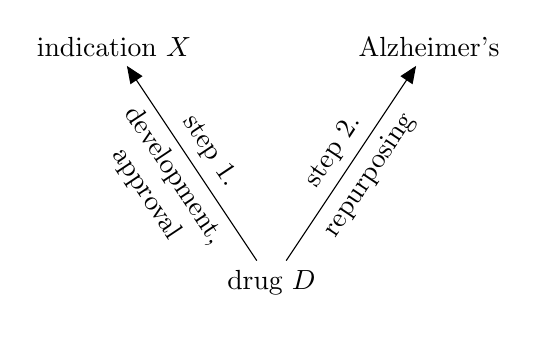
\begin{tikzpicture}
\path (0,0) node (drug) {drug $D$}
	(-2,3) node (ind) {indication $X$}
	( 2,3) node (alz) {Alzheimer's};
\path[->] (drug) edge node[below,sloped,text width=3cm,text centered] {development, approval} node[above,sloped]
	{step 1.} (ind);
\path[->] (drug) edge node[below,sloped] {repurposing} node[above,sloped]
	{step 2.} (alz);
\end{tikzpicture}
\end{column}

\begin{column}{0.4\textwidth}
Approaches to repurposing
\begin{enumerate}
\item shared gene
\item network based
\end{enumerate}
\end{column}
\end{columns}
\end{frame}

\begin{frame}{The network based approach}{Where the shared gene approach fails}
\begin{columns}[t]
\begin{column}{0.35\textwidth}
\begin{center}
PPI toy network

\tiny
Alzheimer's genes:
\tikz{\node[white,circle,inner sep=1pt,fill=red] {B}}
\tikz{\node[white,circle,inner sep=1pt,fill=red] {D}}
\tikz{\node[white,rectangle,inner sep=2.5pt,fill=red] {E}}
\end{center}

\includegraphics[width=\columnwidth]{../../../results/2021-06-14-proximity/toy-proximal-arrow.png}
\end{column}

\begin{column}{0.65\textwidth}

\begin{center}
Applicability
\end{center}
\footnotesize
\begin{tabular}{r|c|c|}
\hline
& \multicolumn{2}{c|}{approach} \\
& shared gene & network based \\
\hline
drug $\rightarrow$ \tikz{\node[white,rectangle,inner sep=2.5pt,fill=red] {E}}& \ding{52} & \ding{52}\ding{52}  \\
drug $\rightarrow$ \tikz{\node[white,rectangle,inner sep=2.5pt,fill=blue] {J}} & \ding{56} & \ding{52}\ding{52} \\
\hline
\end{tabular}
\end{column}
\end{columns}
\end{frame}

\section{Main Section}



\section{Last Section}



\begin{columns}[t]
\begin{column}{0.5\textwidth}

\end{column}

\begin{column}{0.5\textwidth}

\end{column}
\end{columns}


\end{document}
